\documentclass[border=4pt]{standalone}
\usepackage[T1]{fontenc}
\usepackage{helvet}
\renewcommand{\familydefault}{\sfdefault}
\usepackage{graphicx}
\usepackage{caption}
\usepackage{amsmath}
\captionsetup{font={sf,footnotesize},labelfont={sf,bf,footnotesize},justification=justified,singlelinecheck=false}
\begin{document}
\setcounter{figure}{3}
\begin{minipage}{7.20in}
\centering
\begin{figure}[htbp]
    \centering
    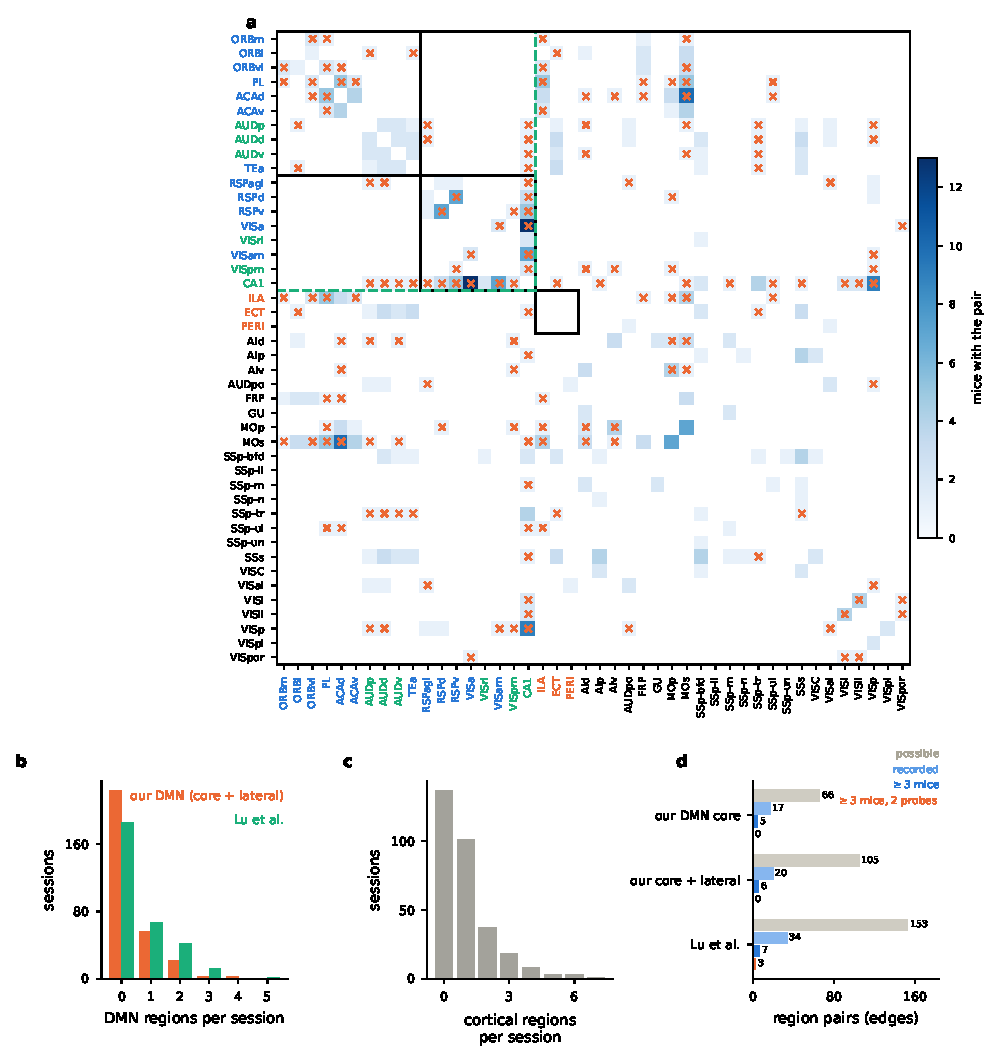
\includegraphics[width=\linewidth]{fig4_coverage_panels.pdf}
    \caption{\textbf{a} Which cortical (and CA1) region pairs have grey-screen co-fluctuation data: number of mice with both regions recorded ($\geq$5 neurons each) in the same session with $\geq$120 still 1 s bins. Of 319 sessions (116 mice) with enough still bins, 308 (114 mice) yield region signals and 104 (70 mice) record at least one such pair. Orange crosses: at least one session records the pair on two different probes. Boxes: the two modules of Lu et al. (prefrontal-temporal, parietal) and the regions only in our DMN (ILA, ECT, PERI; no pair among them is recorded, so that box is empty); dashed green: the full Lu et al. network. Tick colours as in Fig. 3. \textbf{b} Number of DMN regions recorded per session, by definition. \textbf{c} Number of cortical regions recorded per session; most sessions record none or one. \textbf{d} Edges (region pairs) within each DMN definition: possible (light grey), recorded at least once (light blue), recorded in $\geq$3 mice (blue) and recorded on two different probes in $\geq$3 mice (orange), top to bottom. The hub edge of Lu et al., prefrontal (ACA/PL/ORB) to RSP, is recorded in 0 sessions.}
    \label{fig:grey_coverage}
\end{figure}
\end{minipage}
\end{document}
